% document came from
%	https://publishingsupport.iopscience.iop.org/questions/latex-template/
% via 
% 	https://publishingsupport.iopscience.iop.org/journals/physics-education/
\documentclass[12pt]{iopart}
%
\usepackage{graphicx} % needed for figures
%\usepackage{float}
%\usepackage{units}
%\usepackage{hyperref}

\newcommand{\be}{\begin{equation}}
\newcommand{\ee}{\end{equation}}
\newcommand{\bea}{\begin{eqnarray}}
\newcommand{\eea}{\end{eqnarray}}
\newcommand{\degC}{^{\circ}C}
%

\begin{document}
\title[Using Open Source Intelligence Techniques to evaluate Physics Calculations]{Using Open Source Intelligence Techniques to evaluate Physics Calculations}

\author{Physics students (???) and Nathan T. Moore}

\address{
	Physics and General Engineering, 
	Winona State University,
	Winona, MN 55987 USA
}
\ead{nmoore@winona.edu}
\vspace{10pt}
\begin{indented}
\item[\today]
\end{indented}

\begin{abstract}
Checking the answer at the end of a calculation is an oft neglected part of solving physics problems, and getting students to engage in this behavior can be difficult when they are already intellectually tired. 
The paper briefly describes a graphing, linearization, and control of variables activity related to pendulums, couched as ``swingset" design. 
After a reliable $swingtime \sim \sqrt{length}$ model has been established, students apply the model to a youtube video to predict the height of a bridge. 
Then, to reinforce the ideas of multiple representations, and multiple lines of evidence within an argument, students are asked to use Google Maps and other online resources to estimate the height of the bridge. 
Looking for overlap between online estimations and physical models from the lab is powerful. 
At the end of the exercise, students have had a brief introduction to ``Open Source Intelligence" techniques that are commonly used by news and intelligence organizations. 
\end{abstract}

%
% Uncomment for keywords
%\vspace{2pc}
%\noindent{\it Keywords}: XXXXXX, YYYYYYYY, ZZZZZZZZZ
%
% Uncomment for Submitted to journal title message
%\submitto{\JPA}
%
% Uncomment if a separate title page is required
%\maketitle
% 
% For two-column output uncomment the next line and choose [10pt] rather than [12pt] in the \documentclass declaration
%\ioptwocol
%



\section{Swingset Exercise}
Early in a Physical Science or Introductory Physics-Mechanics class, we introduce and practice control of variables, graphing, and linearization concepts by asking students to think about designing a new swingset for an elementary school playground.  
An exciting swingset takes a long time to swing back and forth and we call this ``swingtime" the output variable we want to be able to predict.
Formally, a swingset is typically modeled as a pendulum with period 
$T \sim \sqrt{L}$ \cite{openstax_pendulum, pivot_pendulum} but as this activity usually occurs in the first few weeks of the class, we avoid any mention of the technical story that for small oscillations a pendulum's period is $T\simeq 2\pi \sqrt{L/g}$.

\begin{figure}[h]
\centering
        
\includegraphics[width=\columnwidth]{Fragonard,_The_Swing.jpg}
        %\includegraphics[width=\columnwidth]{2023-05-01.pdf}
        %
\includegraphics[]{Fragonard,_The_Swing.jpg}
\caption{
In North America, a ``swingset" or ``swing" is a mass-rope pendulum system that people enjoy using.
        Swings have had an astonishingly long history of recreational use throughout many human cultures \cite{swings-wikipedia}.
}
\label{buffet}
\end{figure}

When asked about possible input variables on which swingtime might depend, students will often talk about mass, weight, initial height and angle, whether you start from rest or with an initial push, and length.  
After brief investigations, the students typically settle on initial angle, mass, and length as the most important variables needed to predict swingtime.  
With further data collection, the class can narrow down the length of the swing's cable as the most important variable.  

\begin{figure}[h]
\centering
	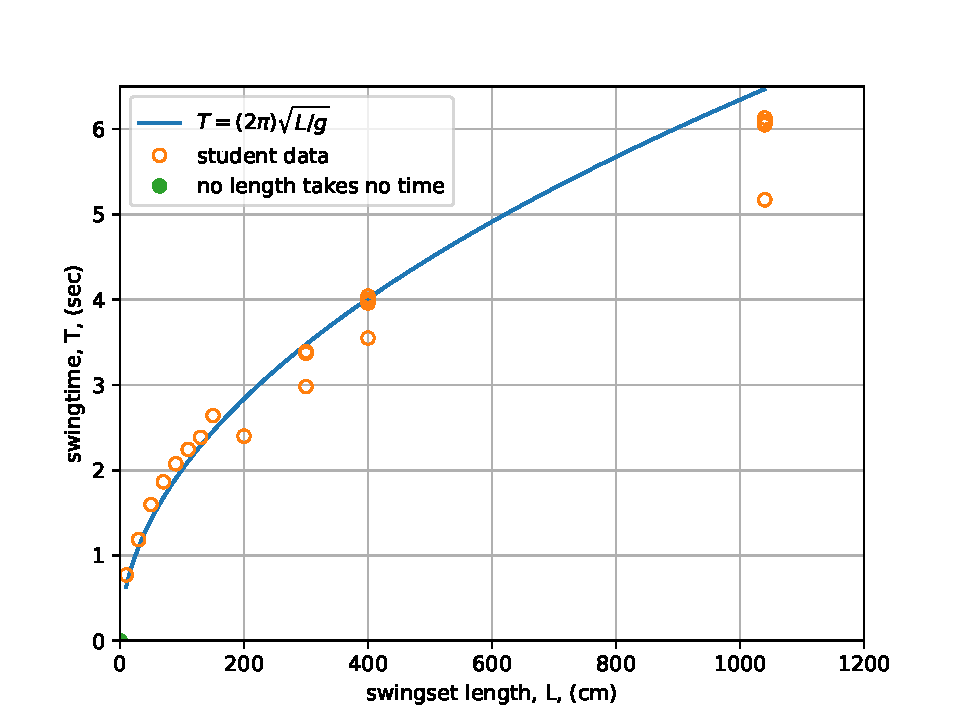
\includegraphics[width=\columnwidth]{linear_swingtime_graph.pdf}
\caption{
Typical student data, using metal washers and string to model the motion of a swingset.
        Students are coached to measure the time associated with multiple ``there and back" swings and then divide to find an average time so that their reaction times (typically $\approx0.3 seconds$) can be ignored.
        }
        \label{swingtime_graph}
\end{figure}

Data from a past class is given in figure \ref{swingtime_graph}. Thus far, all of the students' data has been collected with metal washers and string, with none of the swingsets larger than about $100cm$ in length. The initial data in figure \ref{swingtime_graph} looks fairly linear, and when asked  to predict the swingtime for a $200cm$ length, students typically either draw a line or use a linear math model, also shown in figure \ref{swingtime_graph}.  

This linear model fails at longer swingset lengths. Resolution comes via two pieces of data.  First, if a swingset has ``almost no length" students will generally volunteer that it takes ``almost no time" to swing back and forth.  This means that the $length=0$, $swingtime=0$ intercept is physically real and should be included in fitting efforts.  

Second, when results from swingset lengths of $200cm$, $300cm$ and $400cm$ are included in the graph, students can be coached to recollect that the data reminds them of a parabola that has been rotated to open towards the positive x-axis of the graph.  In Pre-Calculus or Algebra 2 classes this mathematical form is often written as a $y^2=x$ or $y=\sqrt{x}$ relationship.  

To test this ``curvy'' relationship between swingtime and length, we ask the students to create the graph shown in figure \ref{linearized_swingtime_graph} in which the data has been ``linearized'' by plotting $\sqrt{L}$ instead of $L$.  In our experience, many students have not seen a non-linear proportionality ``in the wild'' before, and this can be a challenging concept to discuss -- particularly when thinking about the units involved in linearized trendlines!   

\begin{figure}[h]
\centering
	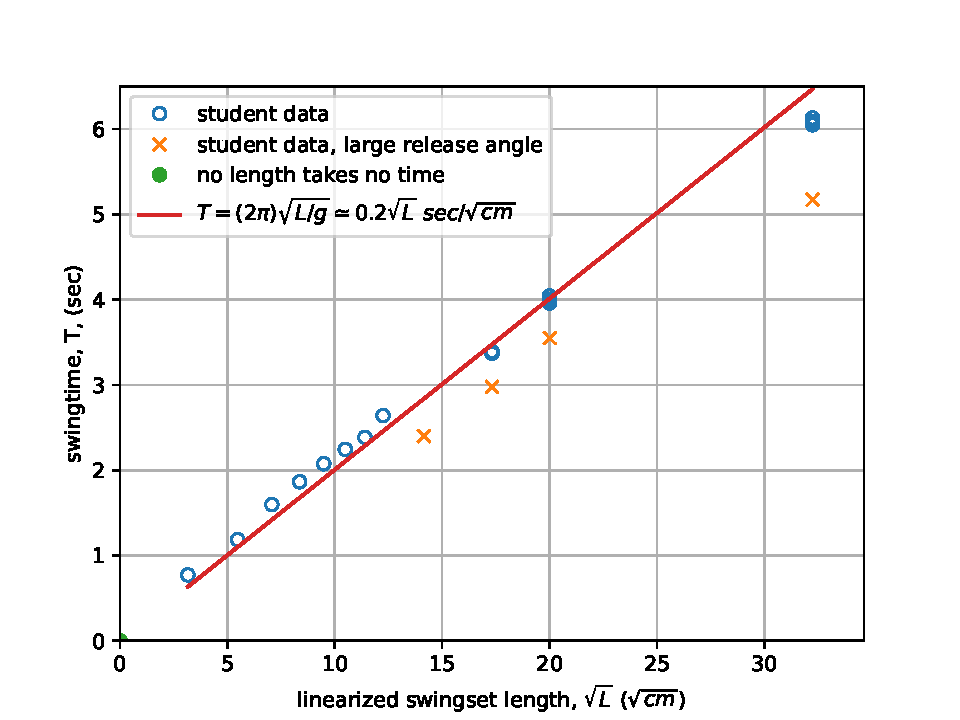
\includegraphics[width=\columnwidth]{linearized_swingtime_graph.pdf}
\caption{
	Linearized swingset data from a class.  Note that $200cm$, $300cm$ and $400cm$ lengths are included and described well by the $\sqrt{L}$ trendline -- so long as the initial release angle is small.  The ``almost no length" swingset that takes ``almost no time" to swing is also nicely included.   
	}
	\label{linearized_swingtime_graph}
\end{figure}

A nice final test of the linearized model for swingtime is to use a $10m$ surveyor's tape measure as a 3-story high swingset.  As seen in figure \ref{linearized_swingtime_graph}, even this data is reasonably described by the linearized model.  Note, most of this work depends on the students using a relatively small initial release angle.  If students decide to release a swingset from horizontal, the $\sqrt{L}$ dependence will be harder to see, which is again visible in figure \ref{linearized_swingtime_graph}.


\section{Predicting the height of a swingset}
With a reliable model for swingsets developed, a common follow-up assignment is to estimate the height of a bridge or arch from video of people swinging below it.  Two specific examples we've used, one in Sault St. Marie, Canada \cite{swingset-sault-ste-marie}, and another near Moab, Utah \cite{swingset-Moab}, are available on youtube.  

At this point, from their data analysis, students know that swingtime, $T$, and swingset length, $L$, are described by an expression similar to the following (with slightly different slopes, depending on student measurements):
\bea
T &\simeq& \left( 0.20\frac{seconds}{\sqrt{cm}} \right) \sqrt{L}, or\\
L &\simeq& \left( 25 \frac{cm}{sec^2} \right) T^2.
\eea
Then, if a student is able to measure the time corresponding to half or a quarter of a swing from the video, they can use the model to predict the swing's height.  As an example, the man in the Sault Ste. Marie video seems to take about 5 seconds to make half a swing (from 0:36 to 0:40 in the video)\cite{details}.  With a period of $T=8s$, students can predict a swingset length of about $1600cm=16m$.  
The video in Moab can be similarly analyzed.   

\section{Evaluating answer using Open Source Intelligence}
This part needs to be written

\subsection{screen grab and scaling}
%Blake Nordby
\textit{This would need to be expanded and illustrated}

While this may be a stretch, the evergreens in the video are roughly shown to be around the same height as the bridge. The average evergreen is between 40-60 feet in height. This, in cm, is between 1219-1828cm. The correlation between the evergreen and my calculation shows that the bridge, with the assumption that the evergreen is of average size, is around 1270cm in height.         For the Moab, because of the way the video is shot (multiple different angles that do not fully show a swing and such), I found it difficult to find another factor to measuring the height of the arch in Moab.

\subsection{geographic searching}
- wrong bridge in Sault St. Marie

\subsection{shadows}


% Anna Becker
\textit{This would need to be expanded and illustrated}

The height of the corona arch is 105 ft. (the arch near moab). This makes sense, considering I calculated the swing to be 95 feet. Which would have the swingers swinging but not crashing into the ground.  

 The height of the bridges shadow was 13 meters 
The height of a shadow of a chevy truck was 2.26 meters  
The height of a chevy truck is around 1.93 meters  

That calculated to make the bridge around 49 feet And I got 42 for my calculation, which is pretty close! 

\subsection{geographic clues}
Moab arches

\clearpage
\section*{References}
\begin{thebibliography}{99}

\bibitem{openstax_pendulum}
College Physics 2e
16.4 The Simple Pendulum
https://openstax.org/books/college-physics-2e/pages/16-4-the-simple-pendulum

\bibitem{pivot_pendulum}
Pivot Interactives Library: Pendulum Investigation
2025 Pivot Interactives, SBC
Version 1.252.0
https://www.pivotinteractives.com/


\bibitem{the_swing_Fragonard}
	https://commons.wikimedia.org/wiki/File:Fragonard,\_The\_Swing.jpg
	Jean-Honoré Fragonard: The Swing 
	1767

\bibitem{swings-wikipedia}
	https://en.wikipedia.org/wiki/Swing\_(seat)
		Swing (seat)

\bibitem{swingset-sault-ste-marie}
https://www.youtube.com/watch?v=arxiDyDouHo
Sault Ste Marie's Biggest Swing Set
Dylan Mcintomney
Oct 29, 2014

\bibitem{swingset-Moab}
https://www.youtube.com/watch?v=4B36Lr0Unp4
World's Largest Rope Swing
devinsupertramp (Devin Graham)
Feb 15, 2012

\bibitem{details} If you download the video from YouTube and import it into Vernier's LoggerPro, it looks like a half swing runs from 36.603s to 39.973s, a $T/2=3.37s$ or $T\approx6.74s$.  
\end{thebibliography}


\end{document}

